\documentclass{article}
\usepackage[utf8]{inputenc}
\usepackage{enumitem}
\usepackage{fancyhdr}
\usepackage{titling}
\usepackage[]{mcode}
\usepackage{amsmath}
\usepackage[T1]{fontenc}
\usepackage{titling}
\usepackage{graphicx} %package to manage images

\graphicspath{ {/images} } %path to images folder

\setlength{\droptitle}{-10em}   % This is your set screw

\def\subject{MACHINE LEARNING AND PATTERN RECOGNITION}
\def\matricno{s1569105}
\def\exmno{B076165}

\title{\subject\\Assignment 1}
\date{November 2015}
\author{Matriculation number - \matricno\\Examination number - \exmno}

\begin{document}

\maketitle
	\section{The Next Pixel Prediction Task}
		\subsection{Data preprocessing and visualization}
			 \begin{enumerate}[label=(\alph*)]
			 	\item
				 	\begin{figure}[htp]
				 		\centering
				 		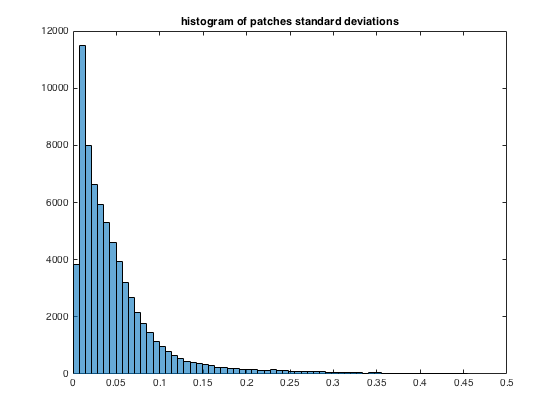
\includegraphics[width=12cm]{images/p1-1-a_std_hist.png}
				 		\caption{histogram of standard deviations in the xtr dataset after normalisation}
				 		\label{fig:p1-1-a_std_hist}
				 	\end{figure}
				 	The maximum possible value of standard deviation is $\frac{max. - min.}{2}$, so in our case after normalisation it is $\frac{1 - 0}{2}= 0.5$. Our threshold to distinguish discrete values of pixels is $\frac{1}{64} = 0.5 / 32 \approx 0.0156$. If we use 32 bins on a range of possible values of standard deviation (between 0 and 0.5) then the width of one bin will be 0.0156 and standard deviations with values  0.0151 or 0.0021 will go to the same bin. But we usually would associate (after rounding using threshold) standard deviation 0.0151 with the discrete (original) pixel value of 1 and 0.0021 with 0 because $round(0.0151/0.0156)=round(0.968)=1$ and $round(0.0021/0.0156)=round(0.135)=0$. Therefore, we must choose minimum 64 bins in order to distinguish such cases because we will have bins width $\frac{0.5}{64} \approx \frac{0.0156}{2} = 0.0078$ and each bin will correspond to the specific discrete (original) pixel value.\\
				 	From the \ref{fig:p1-1-a_std_hist} we can see that after the peak on the second bin the number of patches declines exponentially as  standard deviation increases . We can conclude that most of patches have standard deviation within 0 and 0.05 range, and 0.05 is quite small standard deviation, therefore, most of the patches are flat ones. 
				\item
					I would choose mean of the all the pixels (1032) above and to the left of target pixel as a simplest predictor of the target pixel value for flat patches. In general, I would prefer median because it is more robust to outliers if our dataset is noisy but in our case pixels can take only discrete values and I will show that mean suits us.\\
					Consider extreme case where after normalisation (all pixel values between 0 and 1) in our flat patch  most pixels are zeroes and small portion of pixels are ones (correspond to 63 intensity of original pixel). It is a flat patch so its standard deviation should follow this inequality $\sigma_{flat \, patch} \leq \sigma_{flat \, pach \, max}$. Let $N-m$ be number of zeros and let $m$ be number of ones and I denote $\mu$ as mean. 
					\begin{gather*}
						m < N - m\\
						\mu = \frac{(N - m) 0 + m  1}{N} = \frac{m}{N}\\
						\sigma^2 = (N - m) (0 - \frac{m}{N})^2 + m(1 - \frac{m}{N})^2 \\
						= \frac{(N - m)m^2}{N^3} + \frac{m(N - m)^2}{N ^ 3}\\
						N^3\sigma^2 = Nm^2 - m^3 + mN^2 - 2m^2N + m^3 \\
						= mN^2-m^2N\\
						m^2 - mN + N^2\sigma^2 = 0\\
						m = \frac{N}{2}(1 - \sqrt{1 - 4 \sigma ^ 2})\quad\text{(minus because our case is $m < N - m$ )}\\
					\end{gather*}
					putting $\sigma_{flat \, pach \, max} = \frac{4}{63} \approx 0.0635$ instead of $\sigma$ and using $N = 1032$ we get
					\begin{gather*}
						m = \frac{1032}{2}(1 - \sqrt{1 - 4 * 0.0635^2}) \approx 4.178
					\end{gather*}
					rounding m to the closest integer we receive $m = 4$. \\Thus, in most extreme case of flat patch we can have 4 ones (correspond to original 63 pixel intensity) and 1028 zeros, so it is natural that we want to predict zero as discrete value of our target pixel.  The mean gives us $\mu = \frac{1028 * 0 + 1 * 4} {1032} \approx 0.0038$. Dividing range between 0 and 1 by 64 we get 0.0156 as our threshold to distinguish discrete pixel values. $round(0.0038/0.0156)=round(0.244)=0$ so our mean value will correspond to 0 as the discrete value of our target pixel and that is what we wanted.

			\end{enumerate}		

\end{document}
